\documentclass[a4paper, 12pt]{article}

\usepackage{cmap}
\usepackage{mathtext} 
\usepackage[T2A]{fontenc}
\usepackage[utf8]{inputenc}
\usepackage[english,russian]{babel}	
\usepackage{graphicx,babel,caption,subcaption}
\usepackage{hyperref}

\usepackage{amsfonts,amssymb,amsthm,mathtools}
\usepackage{amsmath}
\usepackage{icomma} 

\usepackage{graphicx} 
\graphicspath{{pictures/}}
\usepackage{wrapfig}

\usepackage{array,tabularx,tabulary,booktabs}
\usepackage{longtable}
\usepackage{multirow}

\usepackage{caption}
\captionsetup{labelsep=period}

% Отступ первого абзаца
\usepackage{indentfirst}
\frenchspacing

\renewcommand{\phi}{\varphi}
\newcommand{\eps}{\varepsilon}

\author{Калинин Даниил, Б01-108а}
\date{23 января 2024 г.}
\title{Магнитный монополь}

\begin {document}

\maketitle

\newpage

\section{Что такое магнитный монополь}
Магнитный монополь -- это теоретическая, предположительно элементарная частица, представляющая собой однополюсный магнит. Существование магнитного монополя было предсказано в 1931 году Полем Дираком. Кстати, в той же работе Дирак предсказал и существование позитрона, позже, после обнаружения в 1932 году, Дирак был удостоен нобелевской премии за это исследование. 

Несмотря на то, что существование монополей прогнозируется теорией великого объединения, в природе они до сих пор не обнаружены. Тем не менее, это не  делает тему менее интересной, ведь, как будет показано далее, магнитный монополь ответил бы на множество вопросов современной физики. Поинтересуемся, какими же свойствами будет обладать магнитный монополь.

\section{Свойства магнитного монополя}
Разберемся, как можно было бы понять, что перед нами действительно магнитный монополь, если вдруг мы его получим. Физика имеет большой опыт определения электрических монополей (то есть зарядов): достаточно просто выстрелить некоторый пробный заряд в сторону исследуемого и наблюдать характерное отклонение. 

Аналогично поступим в случае магнитного монополя. Остается понять, какого рода следует ожидать отклонение, ведь сила, действующая на выстреливаемый электрический заряд будет не так тривиальна.

Схемотично изобразим наш эксперимент на рисунке \ref{fig:experiment}.

\begin{figure}[h]
    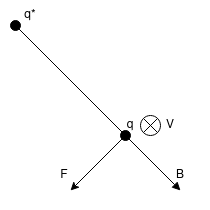
\includegraphics[width=0.4\linewidth]{experiment_setup.png}
    \centering
    \caption{Схема эксперимента по определению монополя}
    \label{fig:experiment}
\end{figure}

Пусть пробный заряд $q$ обладает начальной скоростью $v$ и движется по направлению к неподвижному монополю с "силой" полюса $q^*$. Мы можем проводить эксперименты с меняющимся прицельным расстоянием $b$, т.е. расстоянием между двумя прямыми, параллельными скорости заряда, одна из которых проходит через монополь, а другая -- через заряд. На движущийся заряд действует сила Лоренца, равная

\[
    \vec{F} = q\left[\vec{v}\times\vec{B}\right]
\]

Очевидно, что при расстоянии $b = 0$, скорость заряда будет параллельна одной из линий поля и сила Лоренца не возникнет и, в конце концов, заряд просто столкнется с монополем. Это крайне маловероятный сценарий, поэтому будем считать что $b \neq 0$. 

Поле монополя неоднородно -- его линии расходятся. Чтобы лучше понять происходящее, разобъем скорость в каждый момент времени на тангенциальную и радиальную по отношению к линиям поля компоненты. Первоначально движение будет почти радиальным, поскольку заряд движется на монополь издалека с небольшим прицельным расстоянием. На рисунке \ref{fig:experiment} тангенциальная состовляющая компонента скорости показана стрелкой, направленной за рисунок. Риадиальная же состовляющая не приводит к появлению силы. Сила же, действующая на заряд вследствии тангенциальной состовляющей скорости, также тангенциальная. 

Из таких простых соображений, нам становится ясна первая общая характеристика движения пробного заряда. По мере приближения к монополю движение превращается из поступательного и близкого к прямолинейному во вращательное. При этом должен иметь место переход кинетической энергии поступательного движения в кинетическую энергию вращательного, т.к. магнитное поле не совершает работы. Действительно, сила Лоренца всегда перпендикулярна скорости, поэтому она изменяет только направление, а не величину скорости. Заряд, который изначально приближался к монополю замедляет приближение к нему, начиная вращаться. В некоторый момент поступательная скорость совсем пропадет, и заряд будет только вращаться. Таким образом нами получена вторая общая характеристика движения заряда. По пере того, как заряд приобретает вращательное движение вокруг одной из линий поля, растет отталкивание между зарядом и монополем, что в конечном счете приведет к обратному -- вращательная скорость вовсе исчезнет, зато появится поступательная и заряд полетит в обратном направлении. 

Объединяя все воедино, можно сказать, что заряд будет приближаться к монополю закручиваясь все больше и больше вокруг одной из линий поля, и испытывая отталкивание при этом закручивании. В некоторой точке заряд будет совершать только вращательное движение и, под действием все того же отталкивания начнет удаляться, двигаясь по спирали вокруг той же линии поля. Таким образом, мы ожидаем, что испущенный заряд вернется к нам с той же скоростью, с которой был выпущен. 

В конце работы мы рассмотрим на примере как именно движется заряд в поле монополя.

\section{Монополи в природе}
На самом деле, заголов данного раздела немного обманчив, ведь в природе до сих пор не обнаружили ни единого магнитного монополя. Тем не менее, существуют объекты, которые при определенных условиях ведут себя как монополи. 

Рассмотрим обычный магнитный диполь, например, соленоид. Его поле, как известно, определяется композиция полей магнитных монополей его полюсов:
\[
    B(x) = \frac{\mu_0q^*}{4\pi\left(x - l/2\right)^2} - \frac{\mu_0q^*}{4\pi\left(x + l/2\right)^2}  
\]

Где $l$ -- длина соленоида (плечо диполя).

На расстояниях $x \gg l$, то есть вдали от диполя, выражение упрощается и дает:
\[
    B(x) = \frac{\mu_0 2m}{4\pi x^3}
\]

Где $m = q^*l$ -- магнитный момент диполя.

А теперь самое интересное. Предположим, что $x \ll l$, то есть будем рассматривать поле вблизи одного из торцов соленоида. В основном мы увидим только радиальные состовляющие магнитного поля. Поэтому, хоть монополей и не существует (по крайней мере ни один из них пока не обнаружен) в природе, поведение заряженной частицы в близи торца длинного и тонкого соленоида будет ровно таким, как было описано выше.

Чтобы не показалось, что все сказанное выше -- лишь теоретическая абстракция, можно обратиться к ярокому примеру -- радиационным поясам Ван Аллена. Говоря совсем кратко, американский физик Ван Аллен, запустив вместе с космическим кораблем счетчик Гейгера обнаружил, что землю окружают два радиационных пояса -- внутренний, на радиусах порядка двух земных, и внешний, ограниченный приблизительно восемью земными радиусами. Последующие исследования показали, что частицы (в основном протоны) могут задерживаться в поясе до 10 лет, а их траектории хорошо описываются выкладками из предыдущего пункта. Схематически, радиацонный пояс Ван Аллена и движение частицы в нем изображены на рисунке \ref{fig:van_allen_belt}.

\begin{figure}[h]
    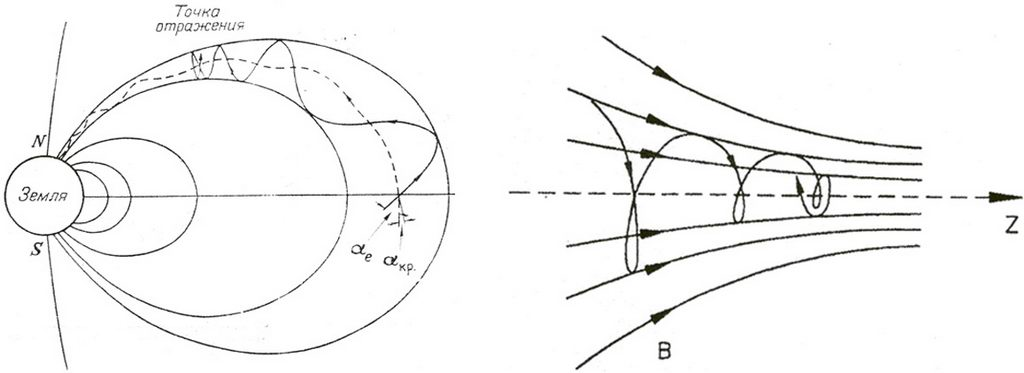
\includegraphics[width=\linewidth]{van_allen_belts.jpg}
    \centering
    \caption{Пояса Ван Аллена и движение частицы в таком поясе}
    \label{fig:van_allen_belt}
\end{figure}


\section{На какие вопросы ответил бы магнитный монополь}
Разобравшись с тем, как мы могли бы обнаружить монополь и какие аналоги монополей существуют в природе, ответим на главный вопрос: "А зачем это все нужно, ведь не было никаких монополей и было все хорошо". 

\subsection{Квантование заряда электрона}
До сегодняшнего дня современная физика не дает ответа на вопрос о квантовании электрического заряда. Известно, что электрический заряд квантуется, но на данный момент это постулируется как экспериментальный факт. Занимаясь этим вопросом, Поль Дирак нашел выражение для "силы" магнитного полюса и показал, что если в природе существует хотя бы один магнитный монополь, то электрический заряд обязательно квантуется. Приведем чуть более наглядное доказательство этого факта, нежели представленное в оригинальной работе.


Прежде всего нужно учесть, что существующие уравнения Максвелла не предусматривают существование магнитных монополей. В своей работе Поль Дирак предложил следующий вариант "исправления" уравнений Максвелла:

\begin{align*}
    div(E) &= 4\pi\rho_e \\
    div(B) &= 4 \pi \rho_m \\
    -rot(E) &= \frac{1}{c} \frac{\partial B}{\partial t} + \frac{4\pi}{c}j_m \\
    rot(B) &= \frac{1}{c} \frac{\partial E}{\partial t} + \frac{4\pi}{c}j_e 
\end{align*}

Здесь введены обозначения $\rho_m$ -- плотность магнитного заряда и $j_m$ -- плотность магнитного тока. Заметим, кстати, что полученные уравнения Максвелла оказываются симметричными.

Рассмотрим следующий эксперимент: монополь с зарядом $q^*$ движется по направлению к сверхпроводящей петле. Тогда в петле будет индуцироваться ток $I$, создающий поле $B$, проходящее через петлю и противоположное полю монополя. Такой ток сохранялся бы в петле достаточно долго после пролета монополя. Заметим, кстати, что после того как монополь прошел через петлю, индуцированный ток все еще будет течь в том же направлении, в отличии от ситуации прохождения диполя через петлю. 

Поскольку весь монополь проходит через петлю, полный магнитный поток монополя должен уравновешиваться полем петли. Вычислим этот поток, обернув монополь сферой радиуса $r$ и воспользовавшись теоремой Гаусса:

\[
    \Phi = \frac{\mu_0 q^*}{4 \pi r^2}4\pi r^2 = \mu_o q^*
\]

В 1961 году было экспериментально обнаружено, что поток через сверхпроводящую петлю с током квантуется и может принимать только значения, кратные некоторому минимальному потоку. В нашей экспериментальной установке прохождение монополя оставляет после себя постоянной ток. Поскольку поток через петлю зависит от величины тока, который в свою очередь вызывается движением носителей заряда, то из квантования потока следовало бы, что квантуется и заряд электрических носителей. Покажем это более формально, воспользовавшись моделью Бора. 

Бор утверждал, что электрон, двигающийся по круговой орбите радиусом $R$ подчиняется условию:

\[
    2\pi R = n \lambda = n \frac{\hbar}{p}  
\]

где $\lambda = \frac{\hbar}{p}$ -- длина волны де Бройля. 

В нашем случае можно считать что носитель заряда -- электрон, двигается по круговой орбите внутри сверхпроводящей петли в однородном магнитном поле $B$. Сила Лоренца будет вызывать центростремительное ускорение:

\[
    evB = m\frac{v^2}{R}  
\]

Комбинируя эти два результата, получим:

\[
    B(\pi R^2) = n \frac{\hbar}{2e}
\]

Таким образом, поток через петлю квантован:

\[
    \Phi = B(\pi R^2) = n \frac{\hbar}{2e}
\]

Квант потока -- флюксон -- очень мал: порядка $10^{-15}~Т\cdot м^2$. В типичной макроскопической системе это не заметно (мы же не рассматриваем каждый движущийся по круговой орбите электрон с точки зрения квантовой механики). Однако сверхпроводники -- особый класс материалов, у которых квантово-механическое поведение становится заметным на макроскопическом уровне. Таким образом, прохождение монополя через сверхпроводяющую петлю вызывает магнитный поток в несколько флюксонов. Современная техника уже может обнаружить такие потоки.

Скомбинируя наши результаты, мы в конечном итоге придем к равенству:
\[
    \mu_0 q^* e = n \frac{\hbar}{2}
\]

Это -- знаменитое равенство Дирака, полученное им в 1931 году. Оно утверждает, как уже говорилось выше, что если в природе существует хотя бы один магнитный монополь, то электрический заряд обязательно квантуется.

Хочется отметить, что в оригинальной статье Дирак выводил свое соотношение через квантование момента импульса. Тем не менее, вывод через квантование потока магнитного поля показался автору несколько более наглядным.

\subsection{Оценка массы монополя}
Оценим массу монополя Дирака, воспользовавшись его соотношением. 

Известно, что энергии электрического и магнитного полей:
\begin{align*}
    W_e &\approx E^2 \\
    W_m &\approx \frac{B^2}{c}
\end{align*}

Т.к. поля электрона и монополя пропорциональны их зарядам, можно дать следующую оценку массы монополя:

\[
    m_m = \frac{q^{*2}}{c^2e^2}m_e  
\]

Используя условие квантования получим окончательно:
\[
    m_m \ge \frac{m_e \hbar^2}{\mu_0 c^2 e^2} \ge 4700m_e  
\]

Таким образом, масса монополя была бы немногим больше двух протонных масс. 

Большой заряд и относительно небольшая масса означают, что монополь Дирака может быть разогнан до огромных скоростей галактическими магнитными полями и затем сильно взаимодействовать с веществом. Предполагается, что если "первобытные" монополи и возникли бы в больших количествах при большом взрыве, то быстрое раздувание вселенной ограничило бы их плотность до ненаблюдаемых значений.


\section{Другие монополи}
Дираковская теория -- не единственная, предсказывающая существование монополей. Наиболее известная из аналогов -- Теория великого объединения, также предсказывает магнитные монополи. Правда, их свойства значительно отличаются от свойств монополей Дирака. Так, масса ТВО-монополей более чем в $10^{16}$ раз превосходит массу монополей Дирака. Это означает, что такие частицы могли бы быть порождены только во время большого взрыва.


% Пусть теперь на монополь Дирака с магнитным зарядом $g$, на расстоянии $b$ от него, движется частица с электрическим зарядом $e$ и скоростью $v$. Сила Лоренца, действующая на эту частицу, будет иметь следующее выражение:

% \[
%     F_{Lorenz} = \frac{ev}{c}B = \frac{eg}{c}\frac{vb}{\left(b^2 + v^2t^2\right)^{\frac{3}{2}}}
% \]

% Тогда частица преобретет импульс $p$ равный

% \[
%     \Delta p = \int{Fdt} = \frac{2eg}{cb}
% \]

% Изменение импульса частицы связано с изменением углового момента
% \[
%     \Delta L = b\Delta p = \frac{2eg}{c}
% \]

% Поскольку орбитальный угловой момент $L = n\hbar$ квантуется, то отсюда вытекает и квантование электрического заряда:

% \[
%     e = \frac{n}{2} \frac{\hbar c}{g},~n=0,~\pm1,~\pm2,~\dots
% \]

% Таким образом, допущение о существовании магнитного монополя объяснило бы квантование электрического заряда (до сих пор остающееся необъяснимым для современной физики).

% Более того, американский физик, лауреат Нобелевской премии, Джулиан Швингер в одной из своих работ показал, что величина элементарного магнитного заряда связана с величиной заряда электрона следующим образом:

% \[
%     g = \frac{137}{2}e
% \]

% В итоге, получаем следующие заключения:

% \begin{itemize}
%     \item  Существование магнитного монополя позволило бы нам объяснить квантование электрического заряда
%     \item Безразмерная константа взаимодействия двух монополей $e$ и $g$ получается очень большой: $g = \frac{137}{2}e$
% \end{itemize}


\section{Симуляция движения заряженной частицы в поле монополя}
Чтобы немного облегчить сухую теорию статьи, автором была подготовлена интерактивная \href{http://139.28.220.13:8501}{симуляция} поведения частицы в поле монополя. Произведенные для расчета выклади достаточно громоздки и опираются на фундаментальную теорему Эмми Нетр, поэтому было принято решение не помещать их в данную работу.

\newpage
 
 
\begin{thebibliography}{}
    \bibitem{}  Arxiv. C. S. Lopez-Monsalvo, A. Rubio-Ponce  -  "Exact trajectories of charged particles in the Dirac
    monopole field"
    \bibitem{}  Журнал Квант. Дж. Вайли  -  "Магнитная монополия"
    \bibitem{}  Arxiv. A. R. Hadjesfandiari  -  "1
    Field of the Magnetic Monopole"
    \bibitem{}  Хабр. [https://habr.com/ru/articles/701910/] Олег Сивченко  -  "Сложный путь к магнитному монополю Дирака"
    \bibitem{}  Хабр. [https://habr.com/ru/companies/ruvds/articles/769962/] - "Могут ли в нашей Вселенной существовать магнитные монополи?"
    \bibitem{} [http://nuclphys.sinp.msu.ru/elp/elp08.htm]

\end{thebibliography}
\end{document}
% \newpage